\section{Central Exclusive $H \rightarrow b\bar{b}$ at ATLAS} 

The aim of this section is to determine whether it is possible to observe the $b\bar{b}$ decay channel of a Higgs boson in central exclusive production at ATLAS. It has already been shown that the $WW^{*}$ decay channel is adequate for discovering the Standard Model Higgs using FP420 for 140~$\leq m_H \leq$~200~GeV \cite{Cox:2005if}. Therefore, in this analysis, the choice of Higgs mass is $m_H = 120$ GeV.

The choice of jet algorithm will affect the reconstructed exclusive variables and hence the choice of cut required to remove the background. The strategy here is to firstly extract the best kinematic matching cuts between the central system and FP420 for each jet algorithm. Further possible exclusivity requirements are then examined in order to reduce the non-exclusive backgrounds. Finally, the cross sections and significance of discovery are presented, along with the impact of possible experimental triggers.

\subsection{Backgrounds}

The backgrounds to the central exclusive $H \rightarrow b\bar{b}$ channel are divided into three categories; central exclusive, double pomeron exchange and overlap. The central exclusive backgrounds are $gg\rightarrow b\bar{b}$ and $gg\rightarrow gg$ and are simulated, along with the Standard Model Higgs signal, using the ExHuME Monte Carlo. The $b\bar{b}$ and $gg$ backgrounds are generated in the mass range $80 \leq M \leq 160$~GeV with a $|\cos\theta| \leq 0.98$ cut in the CM frame. 

%However, equation \ref{exclusivediquark} shows that the exclusive di-quark background is, at a given central mass, strongly peaked in the large pseudo-rapidity region. Hence an $E_T$ and $\eta$ cut will reduce this background. The $gg$ background can be reduced in a similar way. 

The double pomeron exchange processes are simulated using the POMWIG event generator \cite{Cox:2000jt}. As FP420 has acceptance for small values of $\xi$, the processes are generated using the \Pom \Pom \, fusion process without the contribution from the subleading reggeon, which is expected to be small.  POMWIG is normalised to H1 data \cite{Adloff:1997sc} and does not contain a value of the soft survival factor. For the purposes of this analysis, the soft-survival is set to 0.03 \cite{Alekhin:2005dx:Soft}. There are two DPE processes that act as background: $b\bar{b}$ and $jj$, where the $j$ are light quark and gluon jets. These backgrounds have two intact protons in the final state and a jet-like central system. However, the kinematics of the two-jet event measured in the ATLAS detector should not match the kinematics measured in FP420 because of the presence of pomeron remnants in the final state. Section \ref{kinematicmatch} deals with the correct identification of these events.

The overlap background involves two single diffractive (SD) events, which produce the protons measured in FP420, plus a QCD di-jet event all in one bunch crossing at the LHC. The relevant QCD processes are again $b\bar{b}$ and $jj$ and are generated using the HERWIG event generator. However, the protons from the SD events have absolutely no relation to the QCD event and as such, one would expect the kinematics to very rarely match between FP420 and the central ATLAS detector. Furthermore, the protons that gave rise to the QCD event have broken up, which deposits extra energy in the calorimeters and leaves extra tracks in the inner detector. This type of background is covered in more detail in section \ref{overlap}.

\subsection{Jet Algorithm effects and Kinematic Matching Cuts}\label{kinematicmatch}

Starting with just the $H\rightarrow b\bar{b}$ signal events, the two types of jet algorithm were applied. Events  were only retained if the highest transverse energy jet had $E_T > 40$~GeV. This choice is motivated by the transverse energy of the $b$-quarks peaking at 60~GeV if $m_H=120$~GeV (figure \ref{bquarket}) in addition to the  steep transverse energy dependence of the central exclusive backgrounds (figure \ref{dipartonplots} (a)). The effects of the cone and inclusive $K_T$ algorithms on the reconstructed $R_{jj}$
distribution are shown in figure \ref{higgsrjj}.
The $R_{jj}$ distribution has a peak close to 1.0 but a long tail to medium $R_{jj}$ values. This is due to hard final state radiation from one of the $b$ quarks not being recovered by the jet algorithm. The effect of reducing the cone radius results in less of the energy being reconstructed in the two-jet system and a flatter $R_{jj}$ distribution as expected. Reducing $R_{K_T}$ has a similar effect.


\begin{figure} 
\centering
\mbox{
	\subfigure[]{\epsfig{figure=Diagrams/HiggsRJJDiffCone.eps,width=0.5\textwidth,height = 6cm}}
	\subfigure[]{\epsfig{figure=Diagrams/HiggsRJJDiffKTR.eps,width=0.5\textwidth,height = 6cm}}
}
\caption[The effect of the cone and $K_T$ algorithms on the signal $R_{jj}$ distribution]{The reconstructed signal $R_{jj}$ distribution using the cone (a) and $K_T$ (b) jet-finding algorithms. The effect of changing $R_{cone}$ or $R_{K_T}$ is also shown. \label{higgsrjj}}
\end{figure}

In contrast, the variable $R_j$ is defined to be less affected by very hard radiation from one of the jets.
The $R_j$ distribution, shown in figure \ref{higgsrj}, has a narrower peak than the $R_{jj}$ distribution with the long tail removed. Furthermore, changing the jet algorithm parameter has less effect on the distribution -  decreasing $R_{cone}$ or $R_{K_T}$ results in only a small shift to lower values of $R_j$ as progressively more soft particles are not reconstructed in the highest transverse energy jet. This makes $R_j$ a robust variable for defining exclusive events. The $K_T$ algorithm performs slightly better than the cone algorithm because the distribution is less susceptible to changes in $R_{K_T}$. Both algorithms produce similar shapes of distribution.


\begin{figure} 
\centering
\mbox{
	\subfigure[]{\epsfig{figure=Diagrams/HiggsRJDiffCone.eps,width=0.5\textwidth,height = 6cm}}\quad
	\subfigure[]{\epsfig{figure=Diagrams/HiggsRJDiffKTR.eps,width=0.5\textwidth,height = 6cm}}
	%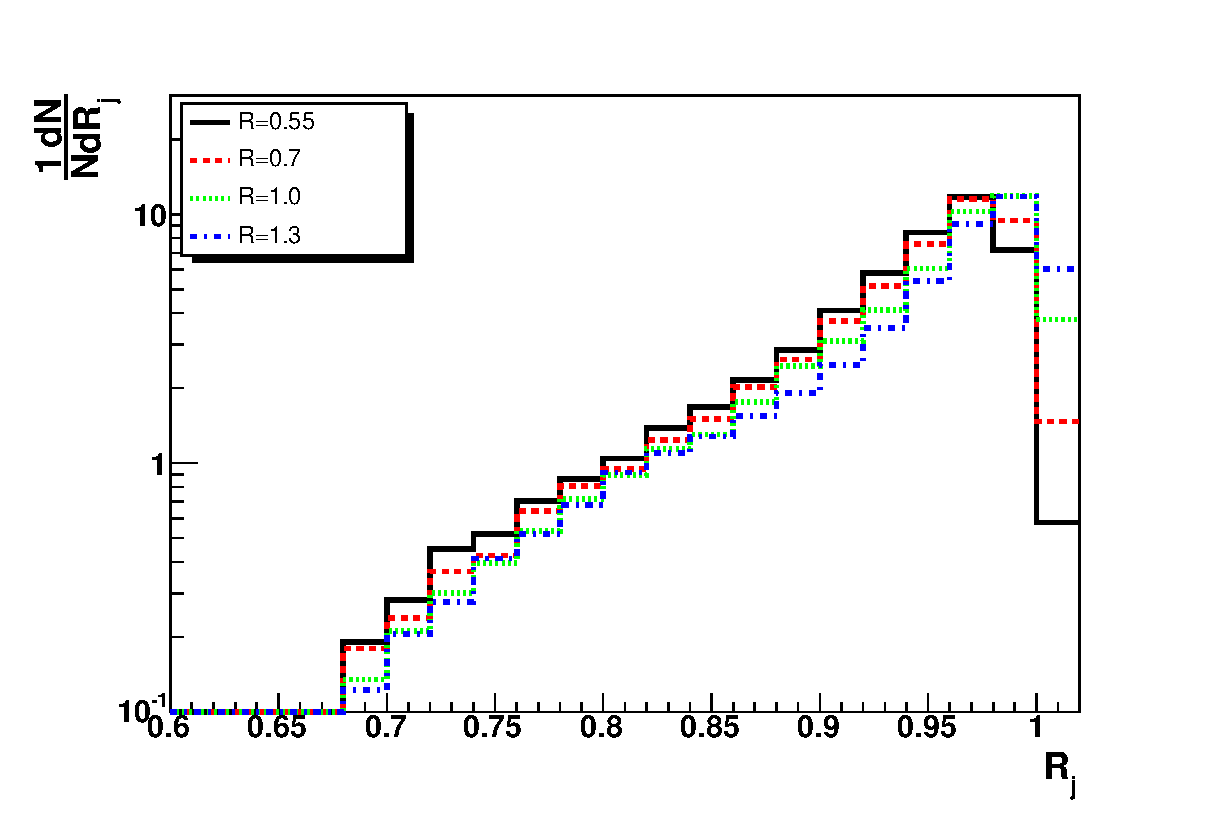
\includegraphics[width=0.5\textwidth]{Diagrams/HiggsRJDiffKTR.eps}
	}
\caption[The effect of the cone and $K_T$ algorithms on the signal $R_{j}$ distribution]{The reconstructed signal $R_{j}$ distribution using the cone (a) and $K_T$ (b) jet-finding algorithms. The $R_j$ distribution less sensitive to changes in $R_{cone}$ or $R_{K_T}$ than $R_{jj}$. \label{higgsrj}}
\end{figure}


The final kinematic matching variable, $\Delta y$, is shown in figure \ref{higgsdeltay}.  Both distributions have the majority of events concentrated in the region $\Delta y < 0.1$. The conclusion is that the $R_j$ and $\Delta y$ variables are extremely good at defining the exclusive event. Furthermore, it is possible to choose small values of $R_{cone}$ or $R_{K_T}$ without too much change in the reconstructed signal. This will be important in high luminosity running at the LHC, where 35 events are expected in every bunch crossing. Smaller values of $R_{cone}$ and $R_{K_T}$ will result in less particles from the pile-up being wrongly added into the jets of interest.

\begin{figure} 
\centering
	\mbox{
	\subfigure[]{\epsfig{figure=Diagrams/HiggsDeltaEtaDiffCone.eps,width=0.5\textwidth,height = 6cm}}
	\subfigure[]{\epsfig{figure=Diagrams/HiggsDeltaEtaDiffKTR.eps,width=0.5\textwidth,height = 6cm}}
	}
\caption[The effect of the cone and $K_T$ algorithms on the signal $\Delta y$ distribution]{The reconstructed signal $\Delta y$ distribution using the cone (a) and inclusive $K_T$ (b) jet-finding algorithms.\label{higgsdeltay}}
\end{figure}

The objective now is to define a set of exclusivity cuts that keep as much of the signal as possible, whilst rejecting a large fraction of the background. The $R_{jj}$, $R_j$ and $\Delta y$ distributions for the central exclusive Higgs are plotted in figure \ref{fig:higgsvsdpebb} against the $b\bar{b}$ background produced via double pomeron exchange. A cone radius of 0.4 and a $K_T$ R-parameter of 0.55 are used, and the distributions are normalised to the same area. It should be noted that, at this stage, the double pomeron exchange $b\bar{b}$ cross section is approximately 380 times larger than the signal although spread over a larger mass range. 

\begin{figure} 
\centering
\mbox{
	\subfigure[]{\epsfig{figure=Diagrams/HiggsvsDPEbb_RJJcone0.4.eps,width=0.5\textwidth,height = 6cm}}\quad
	\subfigure[]{\epsfig{figure=Diagrams/HiggsvsDPEbb_RJJkti0.55.eps,width=0.5\textwidth,height = 6cm}} 
	}
\mbox{
	\subfigure[]{\epsfig{figure=Diagrams/HiggsvsDPEbb_RJcone0.4.eps,width=0.5\textwidth,height = 6cm}}\quad
	\subfigure[]{\epsfig{figure=Diagrams/HiggsvsDPEbb_RJkti0.55.eps,width=0.5\textwidth,height = 6cm}}
	}
\mbox{
	\subfigure[]{\epsfig{figure=Diagrams/HiggsvsDPEbb_DeltaEtacone0.4.eps,width=0.5\textwidth,height = 6cm}}\quad
	\subfigure[]{\epsfig{figure=Diagrams/HiggsvsDPEbb_DeltaEtakti0.55.eps,width=0.5\textwidth,height = 6cm}}
}
\caption[Comparison of the $R_{jj}$, $R_j$ and $\Delta y$ distributions for exclusive Higgs and double pomeron $b\bar{b}$ events ]{The normalised $R_{jj}$, $R_j$ and $\Delta y$ distributions for exclusive Higgs and double pomeron $b\bar{b}$ production, using a cone radius of 0.4 (a, c, e) and inclusive $K_T$ R-parameter of 0.55 (b, d, e).\label{fig:higgsvsdpebb}}
\end{figure}

The values $R_{cone}=0.4$ and $R_{K_T} = 0.55$ are chosen for two reasons. Firstly, they produce similar distributions and do not give a false impression that one algorithm is superior. Secondly, these smaller values of $R_{cone}$ and $R_{K_T}$ are less likely to reconstruct di-jets containing some of the pomeron remnants. This is desirable in order to reconstruct the hard-scattering part of the double pomeron exchange process. The difference between DPE and CEP events is obvious and expected, the presence of pomeron remnants means that the kinematics of the hard sub-process does not match the kinematics measured in FP420.

Using $R_j$ instead of $R_{jj}$ has some interesting effects. Firstly, as expected, the low $R_{jj}$ tail is not present in the $R_j$ distribution for both the signal and background. This initially leads to the presumption that the $R_j$ variable is better at reconstructing the mass of the hard-scatter than $R_{jj}$. However, for the double pomeron $b\bar{b}$ events, the $R_j$ distribution extends to higher values than $R_{jj}$. Some of this increase can be attributed to the highest transverse energy jet containing some pomeron remnant. This extra energy is then counted twice in the $R_j$ reconstruction. This problem is reduced by the use of small values of $R_{cone}$ and $R_{K_T}$ but can never be completely removed.
The second effect of using the $R_j$ variable is that there is a sharper, more distinct separation between the signal and background when compared to the $R_{jj}$ variable. This is mainly due to the long tail in the signal $R_{jj}$ distribution. 

%The $\Delta y$ distribution is also well reconstructed. Smaller values of $R_{cone}$ or $R_{K_T}$ lead to a broader distribution with a long tail to large values of $\Delta y$. This is because hard radiation in the parton showering phase would lead to a significant change in direction of one of the jets if the energy from the radiation is reconstructed as a third jet.

The distributions presented in figure \ref{fig:higgsvsdpebb} give a feel for the loosest possible cuts in those distributions. The loose cut is defined as the point at which the normalised signal and background distributions cross over. For example, a cut of $R_j >$ 0.85 can be applied to di-jets reconstructed using the inclusive $K_T$ algorithm with $R_{K_T}=0.55$. Moving this cut to lower $R_j$ would include a larger fraction of background with only a very small gain in signal. This loose cross-over cut is not the optimum cut for the analysis because the unnormalised background is so much larger than the signal; it only indicates the region of interest for further study. The best cut is determined later by requiring a favourable ratio of signal to all background.
%\afterpage{
%\clearpage

\begin{figure}
\centering
\mbox{ 
	\subfigure[]{\epsfig{figure=Diagrams/ConeDijetMassFractionCut.eps,width =.5\textwidth}}
	\subfigure[]{\epsfig{figure=Diagrams/KTDijetMassFractionCut.eps,width=.5\textwidth}}
	}
\caption[The dependence of the $R_{jj}$ and $R_{j}$ cuts on $R_{cone}$ and $R_{K_T}$]{The dependence of the $R_{jj}$ and $R_{j}$ cuts as a function of $R_{cone}$ (a) and $R_{K_T}$ (b).\label{dijetmasscutsvsparam}}
\end{figure}
%}

The cut value depends on the values of $R_{cone}$ or $R_{K_T}$ used to reconstruct the di-jets. Figure \ref{dijetmasscutsvsparam} shows how the cross-over cut values for $R_{jj}$ and $R_{j}$ change with the jet algorithm parameter. 
Using the $K_T$ algorithm as an instructive example, it is clear that the $R_j$ cut is less dependent on $R_{K_T}$ than the $R_{jj}$ cut. The steep dependence of the $R_{jj}$ cut with $R_{K_T}$ is easily understood, because the signal is reconstructed with larger $R_{jj}$ when $R_{K_T}$ is increased (figure \ref{higgsrjj} (b)). 
Furthermore, the background will also be reconstructed with larger $R_{jj}$ as it is just as susceptible to parton showering. Therefore the cut naturally increases to keep the signal efficiency high and the background efficiency low. A similar effect is found for the cone algorithm, but the dependence is less steep with $R_{cone}$

The $R_j$ cut however, has a weaker dependence on the value of $R_{K_T}$ used to define the jets. Figure \ref{higgsrj} showed that the reconstructed signal shape is almost $R_{K_T}$ independent. The only change is a small shift to larger $R_{j}$ as the value of $R_{K_T}$ is increased. It is natural to assume that the background would follow the same trend. These larger values of $R_{K_T}$ are more likely to pull in some of the remnants, thus the cut increases to keep the background efficiency low. The performance of the cone algorithm is similar across the range of $R_{cone}$ used. 

The $\Delta y$ cut is always less than 0.1 and decreases with $R_{K_T}$ because there is less chance of parton showering changing the direction of a jet.  The cut on $\Delta y$ is not examined further because it is smaller than the granularity of the towers in the hadronic calorimeter. It is not obvious that the direction of a jet can be measured more accurately than the tower granularity and so the exclusivity cut is set at $\Delta y < 0.1$ for the rest of the analysis.

The reconstructed signal and background efficiencies as a function of $R_{cone}$ and $R_{K_T}$ are shown in figure \ref{dijetmasscutefficiency}. For each jet algorithm parameter, the preferred cuts given in figure \ref{dijetmasscutsvsparam} are used. 
For the signal, the performance of the cone and $K_T$ algorithms are similar. In the case of the $R_j$ cut, the efficiency is approximately flat with a slight decrease at large and small values of $R_{cone}$ and $R_{K_T}$. In contrast, the efficiency of the $R_{jj}$ cut increases with both $R_{cone}$ and $R_{K_T}$. This is a direct consequence of the flatter $R_{jj}$ distributions at smaller $R_{cone}$ and $R_{K_T}$, which result in less signal events in the region of interest. In all cases, the best efficiency for signal reconstruction occurs after cuts on the $R_j$ variable. 

%For the signal, the performance of the cone and $K_T$ algorithms are very similar. For $R_j$, the signal efficiency is virtually independent of both $R_{cone}$ and $R_{K_T}$ being flat at about $87\%$. For $R_{jj}$, the efficiency of the signal increases with $R_{cone}$ and $R_{K_T}$. In all cases, the signal efficiency is always better for loose cuts on $R_{j}$ than $R_{jj}$. 

The reconstructed double pomeron background is more interesting. The percentage of events passing the $R_{jj}$ cut decreases as $R_{cone}$ or $R_{K_T}$ increases. This contradicts the expectation that increasing the jet algorithm parameter would result in more of the pomeron remnants being reconstructed in the di-jets for DPE processes.
However, as previously stated, the $R_{jj}$ cut increases with $R_{cone}$ or $R_{K_T}$ because more signal events are reconstructed at high $R_{jj}$. The only explanation is that the improved signal reconstruction cancels the effect of more pomeron remnants being added into the jets. A similar result is found for the cone algorithm when applying an $R_{j}$ cut.

The $K_{T}$ algorithm on the other hand shows completely different dependence for the $R_j$ variable. The percentage of background events passing the $R_j$ cut initially decreases with $R_{K_T}$ if a cut on $R_{j}$ is made. However, at larger values of $R_{K_T}$ the percentage of events passing the cut begins to increase again. The explanation is that, at these larger values of $R_{K_T}$, the probability of pomeron remnants being reconstructed in the highest $E_T$ jet increases, while the signal distribution remains relatively unaffected. The cone algorithm does not show this because the signal $R_j$ distribution changes more with $R_{cone}$ than with $R_{K_T}$ (figure \ref{higgsrj}). 

\begin{figure} 
\centering
\mbox{
	\subfigure[]{\epsfig{figure=Diagrams/ConeDijetMassFractionSignalEfficiency.eps,width =.5\textwidth}}\quad
	\subfigure[]{\epsfig{figure=Diagrams/ConeDijetMassFractionBackgroundEfficiency.eps,width =.5\textwidth}}
	}
	\mbox{
	\subfigure[]{\epsfig{figure=Diagrams/KTDijetMassFractionSignalEfficiency.eps,width =.5\textwidth}}\quad
	\subfigure[]{\epsfig{figure=Diagrams/KTDijetMassFractionBackgroundEfficiency.eps,width =.5\textwidth}}
}
\caption[The efficiency of the $R_{jj}$ and $R_{j}$ cuts as a function of $R_{cone}$ and $R_{K_T}$]{The efficiency of the $R_{jj}$ and $R_{j}$ cuts as a function of $R_{cone}$ and $R_{K_T}$ for the central exclusive Higgs (a,c) and DPE $b\bar{b}$ (b,d) processes.\label{dijetmasscutefficiency}}
\end{figure}

With the small cross sections involved in central exclusive production, it is important to retain as much signal as possible. Furthermore, the cuts should be chosen to minimise the effect of experimental conditions at the LHC. The first point of note is that large values of $R_{K_T}$ and $R_{cone}$ will be more affected by pile-up than smaller values, which implies that smaller values of $R_{cone}$ and $R_{K_T}$ are desirable. With this in mind it is sensible to cut on the $R_j$ variable as the signal efficiency is independent of $R_{cone}$ and $R_{K_T}$. In the case of the $K_T$ algorithm, the natural choice is then to use $R_{K_T} = 0.55$ because this results in the lowest percentage of background events passing the cut (figure \ref{dijetmasscutefficiency} (d)).
 For the cone algorithm, the choice is less straightforward. The plots presented in figure \ref{dijetmasscutefficiency} would indicate that large values of $R_{cone}$ should be used in order to reduce the background by a large value. However, the pile-up issues require small values of $R_{cone}$. As a compromise, the intermediate value of $R_{cone} = 0.4$ is chosen.

The finalised kinematic matching cuts are determined by the jet algorithm parameter and are presented in table \ref{kinematch}. The upper window on $R_{j}$ is chosen after consideration of detector resolution. In \cite{:1999fq:Chapter9}, the offline reconstructed jet resolution was found to be $8.5\%$ for jets with an energy of 50~GeV, which is the approximate energy of the jets in this analysis. The resolution of the $R_j$ variable is dominated by this energy resolution because the FP420 mass resolution is expected to be approximately 2\%. This means that the $R_j$ variable should not be constrained by a window smaller than $0.9<R_j<1.1$, which leaves open the possibility of tightening the lower bounds in $R_{j}$ later if necessary.

\begin{table}[t]
\centering
\begin{tabular}{|c|c|c|}
\hline
Cut & $R_{K_T}=0.55$ & $R_{cone}=0.4$ \\
\hline
$R_{j}^{min}$ & 0.85 & 0.82 \\
$R_{j}^{max}$ & 1.10 & 1.10 \\
$\Delta y$ & 0.1 & 0.1 \\ 
\hline
\end{tabular}
\caption[Kinematic matching cuts to distinguish between the DPE and CEP processes]{The finalised kinematic matching cuts for the cone and $K_T$ algorithms. The $R_j^{min}$ cut was chosen to be the point at which the normalised double pomeron exchange $b\bar{b}$ and central exclusive $H\rightarrow b\bar{b}$ distributions crossed over. The $R_{j}^{max}$ and $\Delta y$ cuts were chosen after consideration of detector effects. \label{kinematch}}
\end{table}%


\subsection{Simulation of the Overlap Background}\label{overlap}

The overlap background is defined as a threefold coincidence of a QCD event and two single diffractive events all in one bunch crossing at the LHC. The overlap background cross section, $\sigma_{\text{olap}}$, can be estimated by 
\begin{equation}\label{overlapxs}
\sigma_{\text{olap}} = \left(N-1\right)\left( N-2\right) \,  P_1 \,  P_2 \, ~Q ~\sigma
\end{equation}
where $N$ is the number of interactions per bunch crossing, $Q$ is the QUARTIC rejection factor and the $P_i$ are the probabilities of an event at the LHC being a single diffractive event that causes a proton hit in FP420.  The labels 1 and 2 indicate the beam to which the single diffractive proton belongs. The input cross section, $\sigma$, is the cross section of the normal inclusive QCD events.

The number of interactions per bunch crossing at the LHC is luminosity dependent and is given in equation \ref{LHCoverlap}. QUARTIC performs the measurement of the time-of-flight difference of the two scattered protons. 
As stated in section \ref{fp420}, this gives a measurement of the interaction vertex to an accuracy of 2.1~mm. In the case of the overlap backgrounds, a fake vertex is reconstructed from the two single diffractive protons. This vertex does not, in general, coincide with the QCD event vertex.

The QUARTIC rejection factor is calculated by picking three random points according to a gaussian distribution of width 5.6~cm, which is the longitudinal beam spot size at the LHC \cite{:1999fq:Chapter3}. Two of these points correspond to the SD vertices and the average corresponds to the fake vertex measured by QUARTIC. If the final point, which corresponds to the primary QCD vertex, is within 2.1~mm of the fake vertex, then the event will pass the QUARTIC measurement. It is found that only 2.5\% of overlap events satisfy this requirement. 
%This is in good agreement with \cite{brandt}.

The $P_i$ are found using the single diffractive cross section, $\sigma_{SD}$, which is given \cite{Khoze:2006gg} by
\begin{equation} \label{sdxs}
\frac{1}{\sigma_T}\frac{d\sigma^{SD}}{dtdx_L} = \frac{g_N^2(t) g_{3\text{\Pom}}}{16\pi^2 g_N(0)}
\left(1 - x_L \right)^{\alpha_{\text{\Pom}}(0) - 2 \alpha_{\text{\Pom}}(t)} S_{SD}^2(s,t)
\end{equation}
where $\sigma_{T}$ is the total cross section, $x_L=1-\xi$ and $g_{3\text{\Pom}}(t) = g_N(0)/3$ is the triple pomeron vertex. 
The soft-survival factor for single diffraction, $S_{SD}^2$, is taken to be 0.085 at the LHC \cite{Khoze:2006gg}. 
The pomeron-nucleon coupling, $g_N(t)$, is given by 
\begin{equation}
g_N(t) = 8 \, \left( \frac{3.52 - 2.79t}{3.52 -t} \right) \frac{1}{\left(1 - \frac{t}{0.71}\right)^2}
\end{equation}
and the Regge trajectory of the pomeron, $\alpha_{\text{\Pom}}(t)$, by\footnote{The actual pomeron trajectory used in \cite{Khoze:2006gg} differs from the standard soft pomeron trajectory of Donnachie and Landshoff \cite{Donnachie:1992ny}. This is necessary in the new approach to both fit the data and account for rescattering corrections. The triple pomeron vertex is also different for similar reasons. The author would like to thank Misha Ryskin for clarification on this issue.}
\begin{equation}
\alpha_{\text{\Pom}}(t) = 1.11 + 0.07t.
\end{equation}
Each $P_i$ is calculated by integrating equation \ref{sdxs} over the FP420 acceptance range for $\xi$ given in section \ref{fp420}. This results is $P_1 = 0.85\%$ and $P_2=0.86\%$. 

The overlap cross section can then be reduced by kinematic matching. The overlap background events are constructed in two steps. The proton $\xi_{1,2}$ and $t_{1,2}$ values are constructed using equation \ref{sdxs} and the Monte Carlo methods presented in section \ref{mcdist}. The values of $t$ are distributed in the range $\{-3,0\}$ and the values of $\xi$ in the FP420 acceptance range.
The QCD event is generated using HERWIG, with JIMMY used for the underlying event  \cite{Butterworth:1996zw}. JIMMY calculates the number of secondary scatters during a proton-proton collision and has two main input parameters: PTJIM specifies the minimum transverse momentum of a secondary scatter and JMRAD(73) specifies the inverse square proton radius. JIMMY has been tuned to Tevatron data \cite{Alekhin:2005dx:MPITune} with PTJIM$=$3~GeV and JMRAD(73)$=$2.13. 

\subsection{Further Exclusivity Requirements}\label{exclusivityreq}

It is now possible to estimate the signal-to-background ratio for central exclusive $H\rightarrow b\bar{b}$ using the following cuts on the MC samples:
\begin{enumerate}
\item The $K_T$ and cone algorithms are used, with $R_{K_T} = 0.55$ or $R_{cone}=0.4$.
\item The highest transverse energy jet must satisfy $E_T > 40$~GeV.  
\item The longitudinal momentum loss of the protons must lie in the FP420 acceptance range,  $0.0023<\xi_1<0.0129$ and $0.0029<\xi_2<0.0171$.
\item The di-jet mass fraction must be in the range $0.85 < R_j <1.10$ for the $K_T$ algorithm or $0.82< R_j <1.10$ for the cone algorithm.
\item The difference between the rapidity of the central system measured by FP420 and the average jet pseudo-rapidity should satisfy $\Delta y < 0.1$.
\end{enumerate}
The first requirement is the choice of jet finding parameter discussed in section \ref{kinematicmatch}. The second cut is motivated by the transverse energy distributions of the Higgs decay products peaking at $\frac{m_H}{2}$. The third cut limits the protons to produce a hit in FP420. The final two cuts reduce the  background by kinematic matching as discussed in section \ref{kinematicmatch}. The subsequent analysis is carried out with both the cone and $K_T$ algorithms, but all the plots presented in this section are for the $K_T$ algorithm unless explicitly stated. The final results are presented for both cone and $K_T$ algorithms.

\begin{figure}
\centering
%\mbox{ 
	\subfigure[]{\epsfig{figure=Diagrams/DeltaRb.eps,width =.5\textwidth}}
%	\subfigure[]{\epsfig{figure=Diagrams/KTDijetMassFractionCut.eps,width=.5\textwidth}}
%	}
\caption[The distance, in $\eta$-$\phi$ space, between the jets and a $b$ quark for a HERWIG $+$ JIMMY $b\bar{b}$ sample]{The distance, in $\eta$-$\phi$ space, of jets with transverse energy greater than 10~GeV from a $b$ quark in the HERWIG $+$ JIMMY $b\bar{b}$ sample.\label{bquarkjets}}
\end{figure}

Potential signal events are those in which the highest two transverse energy jets are tagged as $b$-jets. Because of this, a rudimentary $b$-tagging procedure is applied to the MC samples. For the $b\bar{b}$ samples, a jet is defined to originate from a $b$-quark if the distance
\begin{equation}
\Delta R_{b} = \sqrt{\left(\phi_{j}-\phi_b\right)^2 + \left(\eta_{j}-\eta_b\right)^2}
\end{equation}
between the jet, $j$, and the $b$-quark, $b$, is smaller than a specified amount. Figure \ref{bquarkjets} shows the $\Delta R_{b}$ distribution for the HERWIG $b\bar{b}$ sample using all jets with transverse energy greater than 10~GeV. There is a clear minimum in the distribution and a $b$-jet is therefore defined by $\Delta R_{b} \leq 0.4$. The jets in the $gg$ and light quark samples are assumed to be non $b$-jets.

This designation of jets is necessary because the $b\bar{b}$ final state in the HERWIG samples is often constructed by $gb$ scattering, with the $\bar{b}$ quark produced in the intial state parton shower. In this case, the highest two transverse energy jets will not both originate from $b$ quarks and have a lower probability of being tagged as a $b\bar{b}$ event.
The experimental $b$-tagging efficiency at ATLAS, which is assumed to be 0.6 for a $b$-jet and 0.013 for light quark and gluon jets \cite{:1999fq}, is applied to the two highest transverse energy jets. Thus, each event in the samples is assigned a probability to be tagged as $b\bar{b}$; the tagging probability is 0.36 if the two highest transverse energy jets are both $b$-jets, 0.0078 for $gb$ and $g\bar{b}$ systems and 1.69$\times10^{-4}$ for $gg$ and $jj$.

\begin{table}[tdp]
\centering
\begin{tabular}{|c|c|r|r|}
\hline
Generator & Process & \multicolumn{2}{c|}{Cross section (fb)} \\
& & $R_{K_T}=0.55$ & $R_{cone}=0.4$ \\
\hline
ExHuME & $H\rightarrow b\bar{b}$ & 0.083 & 0.078 \\
 &$b\bar{b}$ & 2.39 & 1.73 \\
 & $gg$ & 3.58 & 1.93\\
POMWIG & $b\bar{b}$ & 3.94 & 2.61\\
& $jj$ & 0.078 & 0.034\\
HERWIG + 2$\times$SD & $b\bar{b}$ & 69.2 & 44.9\\
& $jj$ & 4.52 & 2.57 \\   
\hline
\end{tabular}
\caption[Cross sections of $H\rightarrow b\bar{b}$ and backgrounds after kinematic matching cuts]{The cross sections for signal and background. All samples have had a $E_T > 40$ GeV cut applied to the leading jet and the $b$-tagging procedure applied to the two highest $E_T$ jets. The proton momentum losses were restricted to the FP420 acceptance range  $0.0023<\xi_1<0.0129$ and $0.0029<\xi_2<0.0171$. The cut $0.85<R_j<1.1$ has been applied when using the $K_T$ algorithm. The corresponding cut for the cone algorithm is $0.82<R_j<1.1$, and $\Delta y<0.1$ is applied for both algorithms. The overlap background is defined at a luminosity of $2\times10^{33}$~cm$^{-2}$~s$^{-1}$.\label{inputxs}}
\end{table}%

The cross sections, defined by the cuts at the beginning of this section and scaled by the $b$-tagging procedure, are shown in table \ref{inputxs}. The large $gg$ and $jj$ backgrounds have been significantly reduced by the $b$-tagging. 
The $H\rightarrow b\bar{b}$ cross section is just 0.08~fb and all subsequent cuts are chosen to limit the reduction in the signal. As the overlap background is luminosity dependent, it is quoted at a specific luminosity (2$\times10^{33}$~cm$^{-2}$~s$^{-1}$).

\begin{figure}
\centering
\mbox{
	%\subfigure[]{
	\epsfig{figure=Diagrams/All_Masskti0.55.eps,width =0.75\textwidth}%}
	%\subfigure[]{\epsfig{figure=Diagrams/All_RJAfterCutskti0.55.eps, width =.5\textwidth}}
	}
\caption[The simulated mass distributions of signal and background processes as measured by FP420]{The mass distributions of signal and background processes as measured by FP420. The mass, $M$, has been smeared by a gaussian of width 0.02$M$ to approximate the resolution of FP420. 
\label{massafterkinematics}}
\end{figure}

The backgrounds can be reduced by cutting a mass window around the Higgs peak. The mass distributions for the signal and background are shown in figure \ref{massafterkinematics} after smearing the central mass by a gaussian with a width of 2\%, which simulates the FP420 mass resolution. The background distributions are continuous across the region of interest, thus a mass window of 116~$\leq M \leq$124~GeV is applied to the samples. It is clear that after such a cut, the dominant background comes from the $b\bar{b}$ overlap events. Furthermore, 
%the DPE $b\bar{b}$, the exclusive $b\bar{b}$ and the exclusive $gg$ backgrounds remain larger than the signal. The $jj$ overlap background is approximately the same size as the signal and remains significant.
all of the backgrounds, with the exception of the DPE $jj$ process, remain larger than the signal.

%The $R_j$ distribution, after the cut on the mass measured in the pots, is shown in figure \ref{massafterkinematics}. It is clear that the $R_j$ window will have to be tightened to remove more background.



The overlap background can be reduced further by examining the number of charged tracks associated with the  di-jet vertex. As stated in section \ref{excvars}, an exclusive event only has tracks originating from the hard scatter associated with the primary jet vertex. The overlap events, however, have an inclusive QCD event as the primary vertex. This means that there will be extra particles from the secondary scatters and the break up of the protons. If these particles are charged and lie within the pseudo-rapidity coverage of the inner detector, it will be possible to make a cut on them. The underlying event measures introduced in section \ref{excvars}, $N_C$ and $N_C^{\perp}$, are calculated for charged tracks that have $p_T>0.5$~GeV and lie in the pseudo-rapidity range $|\eta| < 2.5$. The $N_C$ and $N_C^{\perp}$ distributions are shown in figure \ref{nchargedtracks} for the central exclusive Higgs, the DPE $b\bar{b}$ background and the $b\bar{b}$ overlap background. 

\begin{figure}
\centering
\mbox{
	\subfigure[]{\epsfig{figure=Diagrams/All_NChargedkti0.55.eps,width=0.5\textwidth,height = 6cm}}\quad
	\subfigure[]{\epsfig{figure=Diagrams/All_NChargedCDFkti0.55.eps,width=.5\textwidth,height = 6cm}}
	}
\caption[The number of charged tracks associated with the primary vertex]{The $N_C$ distribution (a). Charged particles are defined as tracks if they have $p_T\geq0.5$~GeV and $|\eta|\leq2.5$. Also shown (b) is the $N_C^{\perp}$ distribution which defines tracks that are perpendicular to jets (equation \ref{ncperp}).\label{nchargedtracks}}
\end{figure}

Clearly, the number of charged tracks associated with the primary vertex is a good discriminator for all diffractive events, not just exclusive ones, as shown in figure \ref{nchargedtracks}. 
%These cuts are chose to keep a large signal fraction. 
%It is concluded that the better discriminator is $N_C^{\perp}$ for two reasons. Firstly, the central exclusive distribution is narrower and more sharply peaked at zero. As the measure is intended to measure underlying event, $N_C^{\perp}$ gives a more intuitive result, i.e. that there is no underlying event in central exclusive events. Secondly, the $N_C$ distribution for the overlap background events remains much larger than zero for the majority of the events and the cut will remove the majority of this background.
The signal $N_C^{\perp}$ distribution is narrower than the $N_C$ distribution, which makes it a better measure of the underlying event activity. The $N_C$ distribution suffers because particles that are part of the hard scatter may not be reconstructed in the di-jets by the jet algorithm, hence the broader distribution. However, the $N_C$ distribution covers more of the $\phi$ space and therefore has more chance of picking up activity that is not part of the hard scatter. It is concluded that both cuts are required to remove the overlap background. The tight, underlying event cut, $N_C^{\perp}\leq1,$ is applied first to remove the majority of the background. The looser, $N_C\leq 5$ cut is then applied to the samples to remove events with a large number of particles outside of the transverse region but also outside of the jets.


\begin{figure}
\centering
\mbox{
	\subfigure[]{\epsfig{figure=Diagrams/NChargedBBQCD_pt.eps,width=0.5\textwidth,height = 6cm}}\quad
	\subfigure[]{\epsfig{figure=Diagrams/NChargedCDFBBQCD_pt.eps,width=.5\textwidth,height = 6cm}}
	}
\mbox{
	\subfigure[]{\epsfig{figure=Diagrams/NChargedBBQCD_eta.eps,width=0.5\textwidth,height = 6cm}}\quad
	\subfigure[]{\epsfig{figure=Diagrams/NChargedCDFBBQCD_eta.eps,width=.5\textwidth,height = 6cm}}
	}
	
\caption[The dependence of the $N_C$ and $N_C^{\perp}$ distributions on the minimum transverse momentum and pseudo-rapidity of the charged particles]{The effect on the $N_C$ distribution of $b\bar{b}$ overlap events of changing the minimum transverse momentum that a charged particle can have in order to produce hits in the inner detector (a). Also shown (b) is the effect on the $N_C^{\perp}$ distribution. Both distributions assume particles are detected in the full pseudo-rapidity range of the inner detector. Figures (c) and (d) show the effect on the $N_C$ and $N_C^{\perp}$ distributions of limiting the pseudo-rapidity range of charged particle tracks (with $p_T>0.5$~GeV). All plots are normalised to equal areas. \label{nchargeddependence}}
\end{figure}


The $N_C$ and $N_C^{\perp}$ cuts are dependent on the performance of the inner detector, specifically the lowest transverse momentum a particle can have and still be reconstructed as a track. The effect of changing the minimum transverse momentum on the $N_C$ and $N_C^{\perp}$ distributions is shown in figure \ref{nchargeddependence} (a) and (b). It is important that the inner detector be able to pick up particles with $p_T\simeq0.5$~GeV, otherwise the overlap background could increase by an order of magnitude. Figures \ref{nchargeddependence} (c) and (d) show the effect on the $N_C$ and $N_C^{\perp}$ distributions if the pseudo-rapidity range of the charged tracks is restricted. It is found that limiting the $\eta$ range does not affect the distributions as much as the minimum transverse momentum cut. %This observation is crucial later in the analysis.

\begin{figure}
\centering
\mbox{
	\subfigure[]{\epsfig{figure=Diagrams/All_JetEtakti0.55.eps,width=0.5\textwidth,height = 6cm}}\quad
	\subfigure[]{\epsfig{figure=Diagrams/All_JetPhikti0.55.eps,width=.5\textwidth,height = 6cm}}
	}
\caption[The $\Delta\eta$ and $\Delta\phi$ distributions of the signal and relevant backgrounds]{The $\Delta\eta$ and $\Delta\phi$ distributions of the signal and relevant backgrounds. The $\Delta\eta$ cut is meant to remove the central exclusive backgrounds, whereas the $\Delta\phi$ cut is meant to remove the overlap background.
%% something her on bkgd not put in??
\label{jetdirections}}
\end{figure}

The backgrounds can be further reduced by cutting on the two leading jets, specifically the variables
\begin{equation}
\Delta\eta = | \eta_1 - \eta_2 |
\qquad \text{and} \qquad
\Delta\phi =  \phi_1 - \phi_2 
\end{equation}
where $\eta_i$ and $\phi_i$ are the pseudo-rapidity and azimuthal angle of jet $i$. Figure \ref{jetdirections} (a) shows the $\Delta\eta$ of the signal and some of the backgrounds after the mass window cut. 
A cut on $\Delta\eta$ would remove a large fraction of the signal as well as the background. As the cross section is already small, a cut on $\Delta\eta$ is not made.

The $\Delta\phi$ distributions are shown in figure \ref{jetdirections} (b). The overlap background could be significantly reduced by cutting on $\pi-0.2<\Delta\phi<\pi+0.2$, whilst leaving the signal relatively unaffected.  
 The central exclusive events are back to back in $\phi$ because they have very little overall transverse boost (figure \ref{protonpt} (d)), due to the the $t$ dependence of the cross section. The central exclusive $gg$ distribution is broader than the signal because gluon jets have a larger emission probability and each emission can change the azimuthal angle of the jet. 


Finally, the $R_j$ cut must be tightened as much as possible to remove the DPE background. Figure \ref{rjlast} (a) shows the $R_j$ distribution for the $K_T$ algorithm. The optimum cut to remove 
the DPE events would be $R_j>$0.95. However, the transverse energy resolution of the ATLAS calorimeter again limits the $R_j$ cut and the minimum $R_j$ is therefore set to 0.9. In figure \ref{rjlast} (b), the $R_j$ distribution for the cone algorithm is shown. The cone algorithm reconstructs less DPE events in the large $R_j$ region, which means that the cone algorithm will out perform the $K_T$ algorithm in removing the DPE backgrounds. For both algorithms, the higher emission probability for the gluons results in a higher percentage of $gg$ events being removed by the $R_j$ cut in comparison to the Higgs signal. 

\begin{figure}
\centering
\mbox{
	\subfigure[]{\epsfig{figure=Diagrams/All_RJAfterCutskti0.55.eps,width=0.5\textwidth,height = 6cm}}\quad
	\subfigure[]{\epsfig{figure=Diagrams/All_RJAfterCutscone0.4.eps,width=.5\textwidth,height = 6cm}}
	}
\caption[The $R_j$ distributions after a mass window cut ]{The $R_j$ distribution after a mass window cut (a) for the $K_T$ algorithm with $R_{K_T}=0.55$. Also shown is the same distribution but using a cone algorithm with $R_{cone}=0.4$ (a). \label{rjlast}}
\end{figure}

\subsection{Final Cross Section and Discovery Potential}\label{finalresults}

The efficiency of all the cuts discussed in the previous section are given in table \ref{ktcuteff} for the analysis using the  $K_T$ algorithm. Each cut was chosen to significantly reduce at least one type of background whilst leaving the signal relatively unaffected. The combined cuts let through approximately two-thirds of the signal. For the analysis using the cone algorithm, the distributions are similar, but the optimal cuts are different ($R_j > 0.875$ and $N_C \leq 7$). The efficiency of the cuts for the cone based analysis are shown in table \ref{conecuteff} . In the case of the overlap background, the final $R_{j}$ cut was estimated, for both algorithms, assuming a flat $R_j$ distribution as implied by figure \ref{rjlast}. This was necessary because of the low statistics of the overlap events at this stage of the analysis. The statistical error on the final overlap estimates is approximately 20\%.

The type of jet algorithm has a major effect on the final results. 
The cross sections for the signal and background, after the appropriate cuts, are shown in table \ref{crosssectionfinal}, where the overlap background has been defined at a luminosity of $2\times10^{33}~$cm$^{-2}$~s$^{-1}$.
The $H \rightarrow b\bar{b}$ cross section is 0.057~fb for the $K_T$ algorithm and 0.053~fb for the cone algorithm. The cone algorithm however, outperforms the $K_T$ algorithm in reducing every background and this is shown in the ratio of the cross sections in table \ref{crosssectionfinal}. The important reductions are in the DPE  and $gg$ (CEP) backgrounds. 


\begin{table}[t]
\centering
\begin{tabular}{|cc|c|c|c|c|}
\hline
\multicolumn{2}{|c|}{Process} & \multicolumn{4}{c|}{Cut Efficiency} \\
\cline{3-6}
& & $116\leq M \leq 124$ & $|\Delta \phi - \pi|  \leq 0.2 $ & $N_C^{\perp} \leq 1$ $+$ & $R_j\geq0.9$\\
& & (GeV) & & $N_C \leq 5$ & \\
\hline
CEP & $H$ & 0.905 & 0.920  & 0.836 & 0.982 \\ %
 & $b\bar{b}$ & 0.071 & 0.883 & 0.837 & 0.979 \\ 
 & $gg$ & 0.104 & 0.832 & 0.612 & 0.950\\ %
 \hline
DPE & $b\bar{b}$ & 0.135 & 0.980 & 0.694 & 0.392\\ %
 & $jj$ & 0.117 & 0.944 & 0.617 & 0.351 \\ %
\hline
Overlap & $b\bar{b}$ & 0.104 & 0.363 & $3\times10^{-3}$ &  0.80 \\ %
& $jj$ & 0.102 & 0.332 & $5\times10^{-3}$ & 0.80 \\ 
\hline
\end{tabular}
\caption[Efficiency of cuts for the $K_T$ algorithm]{Efficiency of the optimum cuts for the $K_T$ algorithm ($R_{K_T}=0.55$). The first cut is relative to the cross sections defined in table \ref{inputxs}. Each subsequent cut is then relative to the previous cut in the table. \label{ktcuteff}}
\end{table}%


%\vspace{0.5cm}

\begin{table}[t]
\centering
\begin{tabular}{|cc|c|c|c|c|}
\hline
\multicolumn{2}{|c|}{Process} & \multicolumn{4}{c|}{Cut Efficiency} \\
\cline{3-6}
& & $116\leq M \leq 124$ & $|\Delta \phi - \pi|  \leq 0.2 $ & $N_C^{\perp} \leq 1$ & $R_j\geq0.875$\\
& & (GeV) & & $N_C \leq 7$ & \\
\hline
CEP & $H$ & 0.907 & 0.922 & 0.839 & 0.957  \\
 & $b\bar{b}$ & 0.086 & 0.896 & 0.819 & 0.949 \\
 & $gg$ & 0.133 & 0.884  & 0.531 & 0.649 \\
 \hline
DPE & $b\bar{b}$ & 0.149 & 0.978  & 0.681  & 0.315 \\
 & $jj$ & 0.146 & 0.943 & 0.480 & 0.250 \\ 
 \hline
Overlap & $b\bar{b}$ & 0.099 & 0.392 & 4$\times10^{-3}$  & 0.80 \\
& $jj$ & 0.106 & 0.361& 5$\times10^{-3}$& 0.80 \\
\hline
\end{tabular}
\caption[Efficiency of cuts for the cone algorithm ]{Efficiency of the optimum cuts for the cone algorithm ($R_{cone}=0.4$). The first cut is relative to the cross sections defined in table \ref{inputxs}. Each subsequent cut is then relative to the previous cut in the table.\label{conecuteff}}
\end{table}%



\begin{table}[t]
\centering
\begin{tabular}{|c|c|c|c|c|}
\hline
Generator & Process & \multicolumn{2}{c|}{Cross section (fb)} & $\frac{\sigma_{cone}}{\sigma_{k_T}}$\\
& & $R_{K_T}=0.55$ & $R_{cone}=0.4$ & \\
\hline
ExHuME & $H\rightarrow b\bar{b}$ & 0.057 & 0.053  & 0.93\\ %
 &$b\bar{b}$ & 0.12  & 0.10 & 0.84\\
 & $gg$ &  0.18 & 0.08 & 0.44\\ %
POMWIG & $b\bar{b}$ & 0.14 & 0.08 & 0.57 \\ % 
& $jj$ & 1.9$\times10^{-3}$ & 5$\times10^{-4}$ & 0.26\\ %
HERWIG + 2$\times$SD & $b\bar{b}$ & 0.007 & 0.006 & 0.86\\ %
& $jj$ & 6$\times10^{-4}$ & 4$\times10^{-4}$&  0.67 \\     
\hline
\end{tabular}
\caption[Final cross sections for $H\rightarrow b\bar{b}$ and backgrounds]{The final cross sections for the $H\rightarrow b\bar{b}$ and relevant backgrounds for cone and $K_T$ algorithms. The overlap background is defined at a luminosity of $2\times10^{33}$~cm$^{-2}$~s$^{-1}$. The ratio of the cone to $K_T$  cross sections is also given for each process . \label{crosssectionfinal}}
\end{table}%

Both of these reductions are explained by the fundamental differences of the $K_T$ and cone algorithms. The $K_T$ algorithm reconstructs jets by merging particles that have small transverse momentum with respect to one another. Therefore soft, final state radiation will be reconstructed inside the jets in the case of the $K_T$ algorithm. The cone algorithm on the other hand, will only pull particles into a jet if they lie within the cone radius. Because of this, the $R_j$ and $N_C$ cuts are looser in the case of the cone algorithm to retain as much of the signal cross section as possible. Nevertheless, small cone jets reconstruct less of the $gg$ background in the high $R_{j}$ and low $N_C$ regions as shown in tables \ref{ktcuteff} and \ref{conecuteff}. In the case of DPE, the $K_T$ algorithm has a greater chance of pulling in soft pomeron remnants and therefore reconstructs more of the DPE background in the high $R_j$ region.

The resultant signal-to-background ratio, $S/B$, is calculated to be 0.13 for the $K_T$ algorithm and 0.20 for the cone algorithm using the cross sections presented in table \ref{crosssectionfinal}. This is not constant however, because the overlap cross section increases with luminosity due to the increased number of interactions in each bunch crossing. The signal-to-background ratio is shown as a function of luminosity in figure \ref{StoBvsLumi} (a) and decreases with luminosity. 

\begin{figure}
\centering
\mbox{
	\subfigure[]{\epsfig{figure=Diagrams/StoBvsLumi.eps,width=.5\textwidth, height = 6cm}}\quad
	\subfigure[]{\epsfig{figure=Diagrams/SigvsLumi.eps,width=.5\textwidth,height=6cm}}
	}
\caption[The signal-to-background ratio and significance of the Standard Model Higgs boson as a function of luminosity]{The signal-to-background ratio as a function of luminosity (a). The decrease of the signal-to-background ratio with luminosity is due to the increased overlap background at higher luminosities. Figure (b) shows the significance of discovery per year of running at a particular luminosity\label{StoBvsLumi}}
\end{figure}

Experimentally, the important observable is the number of events that are produced in a given period of time. The number of events is calculated using equation \ref{eventrate}, where the machine luminosity is integrated over the time period of data taking; for example, one year of low luminosity running corresponds to 10~fb$^{-1}$ of data and one year at high luminosity corresponds to 100~fb$^{-1}$. %For a given number of events, $N$, the statistical error is given by $\sqrt{N}$. 
The signal appears as an excess of events over the expected background. The 
%discovery potential is defined as the probability of the background processes to not statistically fluctuate and produce a fake signal. This is measured by the 
significance, $S$, of this excess is a measure of the probability that the predicted background statistically fluctuates to produce a fake signal, and is given by
\begin{equation}
S = \frac{N_s}{\sqrt{N_b}}
\end{equation}
where $N_s$ and $N_b$ are the number of signal and background events respectively. A significance of three is taken to be strong evidence of a new process and a significance of five is defined as a discovery. Usually, results are presented in terms of a significance for a specific amount of integrated luminosity, for example 30~fb$^{-1}$, which corresponds to three years running at low luminosity. In this study however, such a number is meaningless because the overlap background is dependent on the instantaneous machine luminosity. Therefore, the significance for 30~fb$^{-1}$ depends upon whether the data was obtained at low or high luminosity.

Figure \ref{StoBvsLumi} (b) shows the significance per year of running at a specific luminosity. This can be turned into the significance over a longer time period simply by multiplying by $\sqrt{n_y}$, where $n_y$ is the number of years of data acquisition. The cone and $K_T$ algorithms result in a maximum significance of 0.71~yr$^{-1}$ and 0.64~yr$^{-1}$ respectively at a luminosity of $10^{34}$~cm$^{-2}$~s$^{-1}$. However, in terms of significance, the advantage of performing the analysis at high luminosity is not much greater than running at a luminosity of $5\times10^{33}$~cm$^{-2}$~s$^{-1}$, which yields a significance of 0.61~yr$^{-1}$ and 0.54~yr$^{-1}$ for the cone and $K_T$ algorithms respectively. 

The low significance means that the central exclusive  $H \rightarrow b \bar{b}$ is not observable for a Standard Model Higgs using FP420. It would take 18 years of running at high luminosity to get a significance of three, which is simply not feasible. However, as mentioned in section \ref{cephiggs}, a light Higgs boson in the intense coupling region of the MSSM can have an increased cross section for the $b\bar{b}$ decay channel with respect to the Standard Model Higgs boson.

For the rest of this analysis, production of a light Higgs in the MSSM is discussed for the two benchmark points given in section \ref{cephiggs}. The first point (P1) is defined as $M_A=130$~GeV and tan$\beta=$~30, which results in a light Higgs of mass 122.7~GeV with a total decay width of 2~GeV. The second point (P2) is defined as $M_A=130$~GeV and tan$\beta=$~50, which gives a light Higgs of mass 124.4~GeV with a decay width of 6~GeV. The MSSM signal events are created using the ExHuME $H\rightarrow b\bar{b}$ process with an altered decay width to match the MSSM scenarios. The production cross sections are then scaled up using the factors given in section \ref{cephiggs}. 

The backgrounds for both of these benchmark points will increase relative to the Standard Model Higgs analysis due to the large decay width of the Higgs in the intense coupling region of the MSSM. Figure \ref{mssmmass} shows the reconstructed mass, using FP420, of the lightest MSSM Higgs for P1 and P2.  The original mass window of $\pm4$~GeV is no longer sufficient to contain a large fraction of the MSSM Higgs signal and it is necessary to increase the mass window to $\pm6$~GeV for P1 and $\pm10$~GeV for P2. The rest of the cuts applied to the signal and background samples remain the same as the Standard Model Higgs analysis.

%The efficiency of the mass window cut at retaining the Higgs signal is reduced from 90\% for the Standard Model to XX\% at P1 and YY\% at P2. This reduction was necessary because the steep central exclusive $b\bar{b}$ background is increasingly important at lower central masses. Thus the background was regulated by restricting the lower bound of the mass window.

\begin{figure}
\centering
%\mbox{
	\epsfig{figure=Diagrams/MSSMmass.eps,width=.65\textwidth, height = 6cm}
	%\subfigure[]{\epsfig{figure=Diagrams/SigvsLumi.eps,width=.5\textwidth,height=6cm}}
	%}
\caption[The reconstructed mass of the MSSM Higgs]{The reconstructed mass of the MSSM Higgs boson with $m_A=130$~GeV and tan$\beta=30$ (P1) or tan$\beta=50$ (P2). Also shown is the Standard Model Higgs prediction (SM) if $m_H=120$~GeV.\label{mssmmass}}
\end{figure}

The final cross section for the lightest Higgs in the MSSM is  0.132~fb for P1 and 0.316~fb for P2. 
At  low luminosity, only P2 is potentially observable with 3.2 events produced per year at a significance of 1.2 (P1 has 1.3 events per year with a significance of 0.61). Thus P2 would have a significance of 2.94 after six years of data acquisition. At high luminosity, both benchmark points are potentially observable. There would be 13.2 signal events passing the analysis cuts each year for P1, with a significance of 1.5. In the case of P2, there would be 32 events observed every year with a significance of 2.8. P1 would reach a significance of 3 after four years, while P2 would reach a significance of 5.6 after four years.

\subsection{Trigger Considerations}\label{trigger}

The results presented thus far assume a perfect trigger that retains all of the events for the analysis. In reality, this is not the case and the trigger strategy will have an effect on the observable number of events. As the information from FP420 will not be available for the level 1 global decision, the ATLAS detector must be used to retain the event.
The analysis required a jet with a transverse energy greater than 40~GeV in the central detector, which is a triggerable constraint. Unfortunately, jets with such low transverse momentum will not be not retained by the level 1 jet trigger (table \ref{menulvl1}) because the rate for normal QCD events is too large.

Normally, the maximum level 1 rate assigned to jet physics is similar to the level 2 rate, because level 2 does not offer a great deal of additional rejection. In the case of FP420 however, a non-diffractive QCD event will only be retained if there is a coincidence with two SD events in the same bunch crossing. The probability of this threefold coincidence is obtained from equation \ref{overlapxs}, and a large rejective power can be obtained at level 2 by requiring two hits in the forward detectors. 
Furthermore, if QUARTIC is available for the level 2 decision, then the rejection power of FP420 is very large. This is shown in table \ref{fp420lvl2}, where the probability of two hits plus QUARTIC is given for different luminosities.

The standard assumption is that FP420 would be assigned approximately one percent of the level 1 and 2 triggers \cite{Grothe:2006dj}.
As the maximum total event rate at level 2 is approximately 2~kHz, this implies that FP420 will have to reduce the event rate to 20~Hz.  Using the rejection powers given in table \ref{fp420lvl2}, it can be shown that in the worse case scenario of high luminosity and no fast-timing detectors, the level 1 rate could be 240~Hz. If fast-timing is included, the level 1 rate could be as high as 10~kHz at high luminosity. The situation continues to improve at lower luminosities, with a maximum rate of 3~MHz at low luminosity, which exceeds the maximum ATLAS level 1 event rate of 75~kHz. Nevertheless, this implies that a 1~kHz rate at level 1 ($\sim$1\%) does not necessarily have to be imposed if the target is 1\% of the level 2 trigger.

\begin{table}[t]
\centering
\begin{tabular}{|c|c|c|}
\hline
Luminosity & \multicolumn{2}{c|}{Non-diffractive reduction by FP420} \\
($\times10^{33}$) & without QUARTIC & with QUARTIC \\
\hline
1 & 2.7$\times10^{-4}$ & 6.8$\times10^{-6}$ \\ 
3 & 5.8$\times10^{-3}$ & 1.5$\times10^{-4}$ \\ 
5 & 1.8$\times10^{-2}$ & 4.6$\times10^{-4}$\\ 
10 & 8.1$\times10^{-2}$& 2$\times10^{-3}$\\ 
\hline
\end{tabular}
\caption[Non-diffractive rejection power of FP420]{Rejection power of FP420 for the level 2 trigger. The non-diffractive events can only pass the trigger if there has been a threefold coincidence of the primary event with two single diffractive events. The results are given as a function of luminosity with, and without, the use of fast-timing (QUARTIC). \label{fp420lvl2}}
\end{table}%

The total rate for jets with transverse energy greater than 40~GeV will be 25~kHz at low luminosity and 250~kHz at high luminosity \cite{:1999fq:Chapter11,Grothe:2006dj}. In principle, table \ref{menulvl1} shows that it is possible to have such a high jet rate at low luminosity because the predicted total rate at level 1 has a safety margin of 31~kHz. Even without QUARTIC, the FP420 reduction would result in a level 2 jet rate of 5.4~Hz. If this strategy was adopted, all of the events in the analysis would pass the trigger and P2 would be observable after six years as previously stated.

A different trigger strategy at low luminosity would be to utilise the large rapidity gap between the central system and the outgoing proton. Such a trigger would require a lack of hadronic activity in the forward calorimeters and would be susceptible to pile-up events in the same bunch crossing.
Pile-up interactions will be distributed according to Poisson statistics, i.e the probability, $P_n$, of a specific number of pile-up events, $n$, is given by
\begin{equation}
P_n = \frac{\mu^n}{n!}e^{-\mu}
\end{equation}
where $\mu$ is the average number of pile-up events at that luminosity. At low luminosity, the average number of inelastic pile-up events per bunch crossing will be 2.0 and the probability of no inelastic pile-up events accompanying the central exclusive process is calculated to be 13.5\%. Due to the low signal cross-section, one would expect only 0.43 events per year for the P2 scenario. It is concluded that it will not be possible to use a rapidity gap trigger for this analysis at the LHC.

The only other way to trigger the events used in this analysis will be to use the low transverse momentum muon trigger, which requires one muon with $p_T>6$~GeV. 
%As detailed below, up to luminosities of $5\times10^{33}$cm$^{-2}$s$^{-1}$, it may be possible to keep this trigger in conjunction with a jet trigger that requires two jets with transverse energy greater than 40GeV \cite{}. For the rest of the analysis, the luminosity is restricted to be less than  $5\times10^{33}$cm$^{-2}$s$^{-1}$. 
The muon trigger factor for the $b\bar{b}$ events used in this analysis, $f_{b\bar{b}}$, is given by 
\begin{equation}\label{mutrigb}
f_{b\bar{b}}=2P(\mu \, | \, b)
\end{equation}
where $P(\mu \, | \, b)$ is the probability of a $b$-jet containing a muon with $p_T>6$~GeV and the factor of two takes into account that either jet can produce a muon. Using the ExHuME $b\bar{b}$ process, $P(\mu \, | \, b)$ is calculated to be 7.2\% for a minimum $b$ quark transverse energy of $40$~GeV. 

In the case of the $gg$ final state, the muon trigger factor, $f_{gg}$, is given by
\begin{equation} \label{glutrig}
f_{gg} = \frac{2 P(\mu \, | \, g)}{P(b\bar{b} \, | \, g)}
\end{equation}
where $P(b\bar{b} \, | \, g)$ is the probability for the perturbative splitting $g\rightarrow b\bar{b}$ and $P(\mu \, | \, g)$ is the probability for a gluon to produce  a muon with $p_T>6$~GeV. These probabilities were calculated to be 2.8\% and 0.29\% using the ExHuME $gg$ process with a minimum gluon transverse energy of $40$~GeV. The removal of the $P(b\bar{b} \, | \, g)$ factor is necessary because the gluon mis-tag was applied generically to the whole sample in section \ref{exclusivityreq}. The final state muons however, come from the weak decay of $b$ quarks produced in the perturbative splitting and therefore $P(\mu \, | \, g)$ contains $P(b\bar{b} \, | \, g)$. 

Simulation of the ATLAS muon tracker \cite{:1999fq:Chapter11}, shows that it is 80\% efficient at detecting and triggering on muons with transverse momentum greater than 6~GeV. This means, for example, that the muon trigger factor for $b\bar{b}$ events reduces from 0.144 (equation \ref{mutrigb}) to 0.115. The significance per year for the MSSM benchmark points are shown in figure \ref{MSSMsig} with the muon trigger applied. The muon trigger reduces the significance of both P1 and P2 to less than 1.0 per year. This means that an additional trigger is necessary in order to boost the significance in this analysis.

It may be possible to have a low transverse energy jet trigger, which is pre-scaled so that the rate of events passing the trigger does not exceed a specified level.  For example, if a jet rate of 5~kHz is allowed for jets with transverse energy greater than 40~GeV, then the pre-scale factor at low luminosity would have to be 0.2 in order to reduce the total jet rate of 25~kHz. By pre-scaling the jet rate to a fixed value, the total number of events passing this trigger would be constant, regardless of the luminosity. FP420 could then be used to veto the events at level 2, keeping the final jet rate low.

The effect of having a pre-scaled jet trigger, in addition to the muon trigger, is shown in figures \ref{MSSMsig} (a) and (b) for specified level 1 jet rates. The significance per year does not change enough for P1 to become observable and remains below 0.7 in all cases. This corresponds to 18 years of data acquisition to obtain a significance of three. It is concluded that P1 is not observable at ATLAS. P2 on the other hand, has a significance greater than 1.0 per year if the level 1 jet rate is allowed to be greater than 10~kHz. If the level 1 jet rate is allowed to be 25~kHz, then there would be 5 events produced every year, with a significance of 1.35, at a luminosity of 5$\times10^{33}$~cm$^{-2}$~s$^{-1}$. This corresponds to a significance of 3.0 after five years of data taking. It is concluded that the P2 is observable, but only if a pre-scaled jet trigger is developed at  ATLAS.

\begin{figure}
\centering
\mbox{
	\subfigure[]{\epsfig{figure=Diagrams/SigMSSMP1.eps,width=.5\textwidth, height = 6cm}}\quad
	\subfigure[]{\epsfig{figure=Diagrams/SigMSSMP2.eps,width=.5\textwidth,height=6cm}}
	}
\caption[The significance of MSSM Higgs production in the intense coupling region after proposed ATLAS triggers]{ The significance of light Higgs production for the benchmark points P1 (a) and P2 (b).  
The triggers are defined as one muon with transverse momentum greater than 6~GeV (MU6) or a jet trigger for $E_T> 40$~GeV which is pre-scaled to give a maximum level 1 rate of 5~kHz, 10~kHz or 25~kHz. For 5~kHz, typical pre-scales are 0.2 at low luminosity and 0.02 at high luminosity.
\label{MSSMsig}}
\end{figure}

The low transverse momentum muon trigger is strictly only applicable at low luminosities. However, at higher luminosities, this trigger can be viewed as an additional veto on low transverse energy jets. The total rate, $R$, for one jet with transverse energy greater than 40~GeV and a muon with $p_T>6$~GeV can be estimated by
\begin{equation}
R =  2\left[ \, P(\mu \, | \, g) \frac{\sigma_g}{\sigma_{jets}} \, 
+ \, P(\mu \, | \, c )\frac{\sigma_c}{\sigma_{jets}} \, 
+ \, P(\mu \, | \, b)\frac{\sigma_b}{\sigma_{jets}} \, \right] R_{jets}
\end{equation}
where $\sigma_{jets}$ is the total jet cross section for jets with transverse energy greater than 40~GeV and $\sigma_g$, $\sigma_c$ and $\sigma_b$ are the light quark/gluon, $c$ and $b$ jet cross sections respectively. $R_{jets}$ is the total rate for jets with transverse energy greater than 40~GeV.  $P(\mu \, | \, c )$ is the probability for a $c$ jet to contain a muon with $p_T>6$~GeV and is calculated to be 3.3\% using the ExHuME $c\bar{c}$ process with a minimum $c$ quark transverse energy of $40$~GeV. 

The jet cross sections are calculated using HERWIG with a minimum parton transverse energy of 40~GeV. The total jet cross section is found to be 48~$\mu$b and the $c$ and $b$ jet cross sections are found to be 2.2~$\mu$b and 1.5~$\mu$b respectively. The total jet rate scales from 25~kHz at low luminosity to 250~kHz at high luminosity, which gives a final rate for a muon plus jet trigger of 0.323~kHz at low luminosity and 3.23~kHz at high luminosity. This trigger would therefore be allowed up to 3$\times10^{33}$~cm$^{-2}$~s$^{-1}$ if the rate is constrained to be $\sim$1\% of the total level 1 rate. However, as FP420 has a large rejection power at level 2, this trigger could be allowed at high luminosity if a larger percentage of the level 1 rate is allowed.


\subsection{Uncertainties on the Cross Section}\label{higgsxsuncertainties}

%intro to uncertainty
In this section, the uncertainties on the results given in section \ref{trigger} are discussed. 
The central exclusive processes all suffer from uncertainties associated with the calculation of the luminosity of the incoming gluons given in equation \ref{ceplumi}. As shown in figure \ref{exhumelumi}, there is a 50\% uncertainty from the choice of parton density function.  The Durham group estimate \cite{DeRoeck:2002hk} that the soft survival factor is accurate to 50\% and that NLO contributions to the Sudakov suppression result in a  20\% uncertainty. Non-perturbative effects are estimated to contribute another 50\% uncertainty to the calculation. This results in an overall factor of 1.9  uncertainty in the calculation of the luminosity of the incoming gluons.  
For the hard subprocesses, the Durham group estimate that NNLO corrections to the $gg \rightarrow H$ vertex introduce a 25\% uncertainty in the Higgs cross section. No higher order corrections to the CEP $b\bar{b}$ and $gg$ cross sections have yet been published.

%%CEP uncertainties. done

The main uncertainty for the double pomeron exchange processes comes from the modelling of the pomeron in the POMWIG event generator. The first issue is the choice of diffractive PDF that should be used. POMWIG implements two fits, known as H1 Fit 2 and H1 Fit 3 \cite{Adloff:1997sc}. The results presented in section \ref{finalresults} were obtained using the H1 Fit 2 diffractive structure function, which is the default in POMWIG. %H1 Fit 3 however, has a peaked gluon at high $\beta$ \cite{} and would therefore increase the final DPE cross section because the di-jets would contain more of the missing mass.
If H1 Fit 3 was used however, the final DPE cross section would increase because Fit 3 has a peaked gluon at high $\beta$ and more DPE events would therefore be reconstructed in the high $R_{j}$ region.
Fit 3 however, has recently been ruled out by the H1 Collaboration \cite{unknown:2006hx}, which finds a steadily falling gluon distribution at larger values of $\beta$. 

%Another choice when using the POMWIG event generator is the treatment of the pomeron remnants. 
POMWIG also allows the user to define the valence partons in the pomeron to be either quarks or gluons. The default setting is that the valence partons are gluons, which is motivated by the observation that the pomeron is mainly a gluonic object. In the case of di-jet production which is considered here, the partons entering the hard scatter are most likely to be gluons. However, if the valence partons are defined to be quarks, the HERWIG initial state parton shower will be forced to continue until a $q\bar{q}$ pair is produced. This increases the activity in the remnant sector and high $\beta$ values are less likely. The effect of using valence quarks is to decrease the DPE $b\bar{b}$ cross section (using a cone algorithm of radius 0.4) from 0.08~fb to 0.01~fb. This should be considered a lower bound on the calculated cross section, and the realistic cross section should lie in the range 0.01 - 0.08~fb.

The first source of uncertainty for the overlap background is the number of pile-up events at each luminosity. The cross section of two single diffractive events plus a hard scatter is given by equation \ref{overlapxs}, which has a square dependency on the number of interactions per bunch crossing. The average number of interactions, for a specific machine luminosity, is given by equation \ref{LHCoverlap} and is dependent on the total cross section at the LHC. As the total cross section is predicted to be $111.5^{+3.7}_{-11.1}$~mb, the overlap background estimate is accurate to ($+12.4$, -$37.1$)\% at low luminosity and ($+6.9$, $-20.9$)\% at high luminosity. 

The second source of uncertainty on the overlap background comes from the underlying event model used in the analysis. The JIMMY parameters are tuned so that HERWIG reproduces existing Tevatron data. However, it was found \cite{Alekhin:2005dx:MPITune} that two different tunings can be used to describe the data. In this analysis, Tune A was used (PTJIM=3.0, JMRAD(73)=2.13), which predicts more underlying event activity at the LHC than Tune B (PTJIM=2.0, JMRAD(73)=0.71). 
Tune A was chosen because it gives a slightly better description of the Tevatron data.
If Tune B is used however, the effectiveness of the charged particle multiplicity cuts at removing the overlap background decreases from 99.6\% to 99.3\%. This increases the overlap background by a factor of 1.75, which implies an additional uncertainty of $+75$\% on the overlap background. 

The final source of uncertainty comes from the effect of pile-up on the charged track multiplicity cut. The problem is that charged tracks from pile-up events could be identified with the primary event. Experimentally, one would define a vertex window around the primary event vertex and the size of the window would depend on two factors: the severity of the pile-up and the vertex resolution of charged tracks in the inner detector. An attempt is made here to qualitatively estimate the effect on the signal and background.

Firstly, the charged track vertex resolution, $\sigma_z$, of the inner detector limits the vertex window size, $v$, to be
\begin{equation} \label{vertexsize}
v \approx \pm 2\sigma_z
\end{equation}
in order to keep the effectiveness of the charged particle multiplicity cuts. The vertex resolution, given in equation \ref{trackrec}, is dependent on the transverse momentum and pseudo-rapidity and will be less accurate if either $p_T$ is small or $|\eta|$ is large. Figures \ref{nchargeddependence} (a) and (b)  showed that the detection of particles with low transverse momentum particles is essential if the multiplicity cut is to be fully effective. However figures \ref{nchargeddependence} (c) and (d) showed that narrowing the pseudo-rapidity range of the particles had a smaller effect on the multiplicity distributions. This is important because the vertex resolution for particles with $p_T>0.5$~GeV is 0.59~mm, 1.31~mm and 3.61~mm for pseudo-rapidities of 1.0, 1.75 and 2.5 respectively. It is possible therefore, to restrict the pseudo-rapidity range to $|\eta| < 1.75$ in order to have a smaller vertex window in accordance with equation \ref{vertexsize}. If the particle range is restricted to $|\eta|<1.75$, the overlap backgrounds increase by a factor of 1.5. This gives an error of $+50\%$ on the overlap backgrounds from the unknown vertex size.

\begin{figure}[t]
\centering
	\epsfig{figure=Diagrams/NChargedProbability.eps,width=.65\textwidth,height=6cm}
	
\caption[The probability of an inelastic pile-up event being within a given distance of the primary vertex]{The probability, $P$, of an inelastic pile-up event being within a given distance, $\pm \delta$~mm, of the primary vertex. The pile-up events were distributed by a gaussian with a width of 5.6~cm, which is the longitudinal beam spot size at ATLAS.\label{probpileupvertex}}
\end{figure}


The effect of tracks from inelastic pile-up and the optimisation of the vertex window could only be accurately calculated with full detector simulation. However, figure \ref{probpileupvertex} shows the probability, $P$, of an inelastic pile-up event falling within a given distance, $\delta$, of the primary vertex. The $\delta=\pm2.6$~mm curve corresponds to an inelastic pile-up event falling within a vertex window defined for particles with $|\eta|<1.75$. The majority of these events will affect the charged multiplicity cut and so $(1-P)$ is a good estimate of the number of events unaffected by inelastic pile-up. This implies that more than 70\% of events will continue to pass the charged multiplicity cut at a luminosity of 5$\times 10^{33}$ cm$^{-2}$ s$^{-1}$. The $\delta=\pm7.2$~mm shows the probability of a pile-up event falling within the vertex window if all charged tracks in the inner detector are used for the multiplicity cut, i.e $|\eta| < 2.5$. In this case only 40\% of events would pass the charged particle multiplicity cut at a luminosity of 5$\times 10^{33}$ cm$^{-2}$ s$^{-1}$, which shows the importance of determining the optimal vertex window size.
For the rest of the discussion, a vertex window of $\pm2.6$~mm is assumed to be optimal. 

Each of the uncertainties discussed in this section produces an uncertainty in the discovery potential of the MSSM benchmark point P2. The uncertainty in significance (per year of data acquisition) due to the central exclusive processes is shown in figure \ref{uncertaintybounds} (a). As the central exclusive processes dominate both the signal and background cross sections, one would expect that they would also dominate the uncertainty in significance.


\begin{figure}[t]
\centering
\mbox{
	\subfigure[]{\epsfig{figure=Diagrams/MSSMCEPbounds.eps,width=.5\textwidth,height=6cm}}\quad
	\subfigure[]{\epsfig{figure=Diagrams/MSSMbounds.eps,width=.5\textwidth,height=6cm}}
	}
\caption[The uncertainty bounds on the significance of MSSM benchmark point 2]{The uncertainty bounds due to the central exclusive processes (a) on the significance of P2. The triggered events either have a muon with $p_T$ greater than 6~GeV or pass a pre-scaled jet trigger of $E_T>40$~GeV. The pre-scale factor was chosen to limit the total inclusive jet rate to 25~kHz regardless of luminosity. At high luminosity, this corresponds to a pre-scale factor of 0.1. Figure (b) shows the total uncertainty due to all processes. The upper limit is almost unchanged. The lower limit reduces slightly due to the larger overlap background.\label{uncertaintybounds}}
\end{figure}

Figure \ref{uncertaintybounds} (b) shows the total uncertainty in significance. The total uncertainty was estimated by calculating the change in significance due to each individual uncertainty and adding the results in quadrature. It is clear from figures \ref{uncertaintybounds} (a) and (b)  that the central exclusive  uncertainty dominates the range in discovery potential as expected. Furthermore, this large uncertainty in significance has a major effect on the discovery potential. The upper bound of the uncertainty, with a significance of 2.1 per year of data acquisition at a luminosity of 5$\times10^{33}$~cm$^{-2}$~s$^{-1}$, would reach a significance of 3.0 after just two years. Conversely, the lower bound in significance is always less than 1.0 per year and would not be observable using the ATLAS detector.


 
 
